\chapter{Conceitos Básicos}

Aprendizado de máquina é um dos campos de pesquisa da inteligência artificial e por sua vez da ciência da computação.
Esta área de estudos se concentra na pesquisa e desenvolvimento de algoritmos de aprendizado que possam aprender tarefas automaticamente.
Tipicamente estes algoritmos geram um \textit{modelo matemático} partir de um ou mais conjuntos de dados.
O modelo é então responsável por desempenhar a tarefa, ou seja, não é necessário escrever um programa para tanto.
Aprendizado de máquina tem inúmeras aplicações, entre elas podemos citar filtros de spam, reconhecimento ótico de caracteres, motores de busca, \textit{computer vision}, etc.

\section{Aprendizado Supervisionado}

Aprendizado supervisionado é inspirado na ideia de aprendizado por exemplos.
Isto é, uma grande quantidade de exemplos é fornecida para o algoritmo no intuito de faze-lo aprender.
Todos os exemplos devem ter o mesmo formato.
Cada um deles é composto por dois ou mais atributos, sendo que um dos atributos deve ser o alvo da tarefa de aprendizado.
Os demais atributos devem constituir informações relevantes que permitam ao algoritmo aprender a tarefa.
De forma geral temos que um conjunto com \textit{N} exemplos é da forma $ \{(x_1, y_1), ..., (x_N,\; y_N)\} $ tal que $x_i$ representa o conjunto de atributos informativos do exemplo e $y_i$ é seu atributo alvo.

\begin{figure}[h!]
  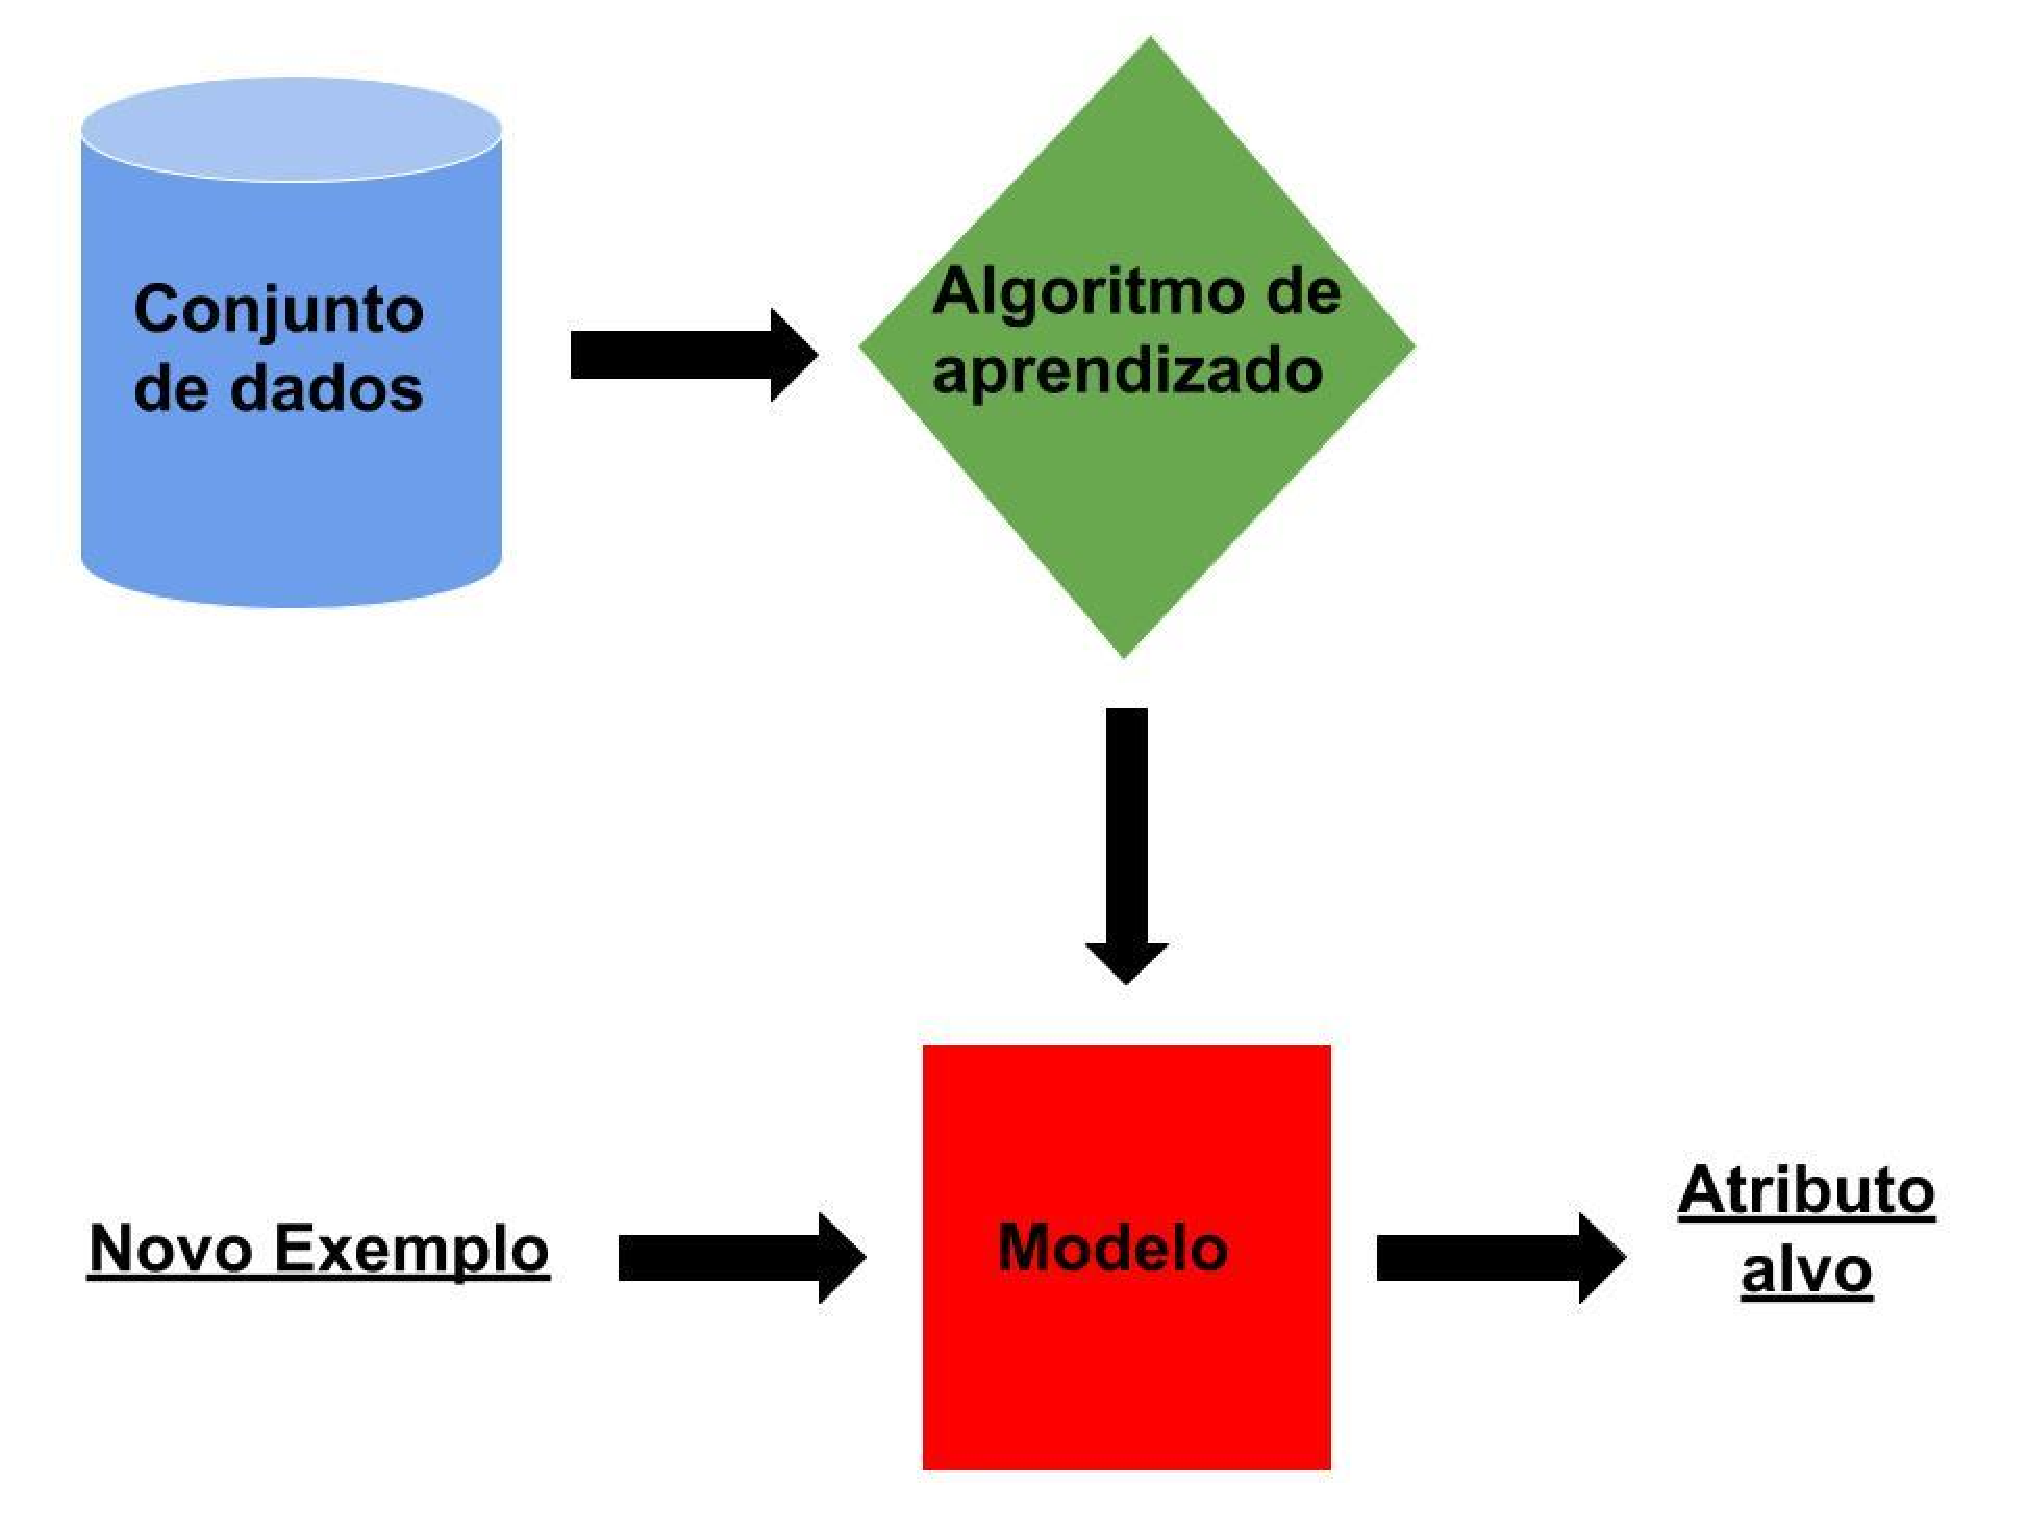
\includegraphics[width=\linewidth]{images/conceitosbasicos01.eps}
  \caption{Fluxo do aprendizado supervisionado para classificação}
  \label{fig:conceitosbasicos01}
\end{figure}

O algoritmo de aprendizado deve gerar uma função $g: X \to Y$, onde \textit{X} é o conjunto de entrada e \textit{Y} o conjunto de saída.
Uma vez que processou os exemplos, o algoritmo gera um modelo que representa a função \textit{g}.
Por fim, dados que ainda não foram vistos, desprovidos do atributo alvo, podem ser submetidos ao modelo.
Com isso, ele pode executar automaticamente a tarefa para a qual foi treinado, e.g. determinar a qual classe o dado inédito pertence.
Veja na figura \ref{fig:conceitosbasicos01} um diagrama que ilustra o processo de aprendizado supervisionado.

Para exemplificar como funciona o aprendizado supervisionado, consideremos o problema da figura \ref{fig:conceitosbasicos02}.
Neste queremos um modelo capaz de diferenciar entre círculos e triângulos.
Ou seja, temos um problema de classificação binária.
Para resolve-lo precisamos de um modelo que funcione como um separador linear.
O algoritmo utilizado para gerar o modelo deve então aprender uma função \textit{f(x)} que mapeia o vetor de entrada \textit{x} em um único valor de saída. Esta função pode ser definida como:

\begin{equation*}

f(x) =
	\begin{cases}

	1 & \text{se }w \cdot x + b > 0\\
	0 & \text{caso contrário}

	\end{cases}

\end{equation*}

onde,
\begin{itemize}
\item Os valores de saída de \textit{f(x)} representam a resposta do classificador, por exemplo o valor 0 pode indicar um círculo e o valor 1 um trigângulo
\item \textit{x} é um vetor de números reais que representam os valores de atributos de entrada, no exemplo são as coordenadas de cada círculo e triângulo
\item \textit{w} é um vetor de números reais que representam os pesos conferidos aos atributos pelo algoritmo de aprendizado
\item \textit{b} é uma constante de bias
\end{itemize}

\begin{figure}[h!]
  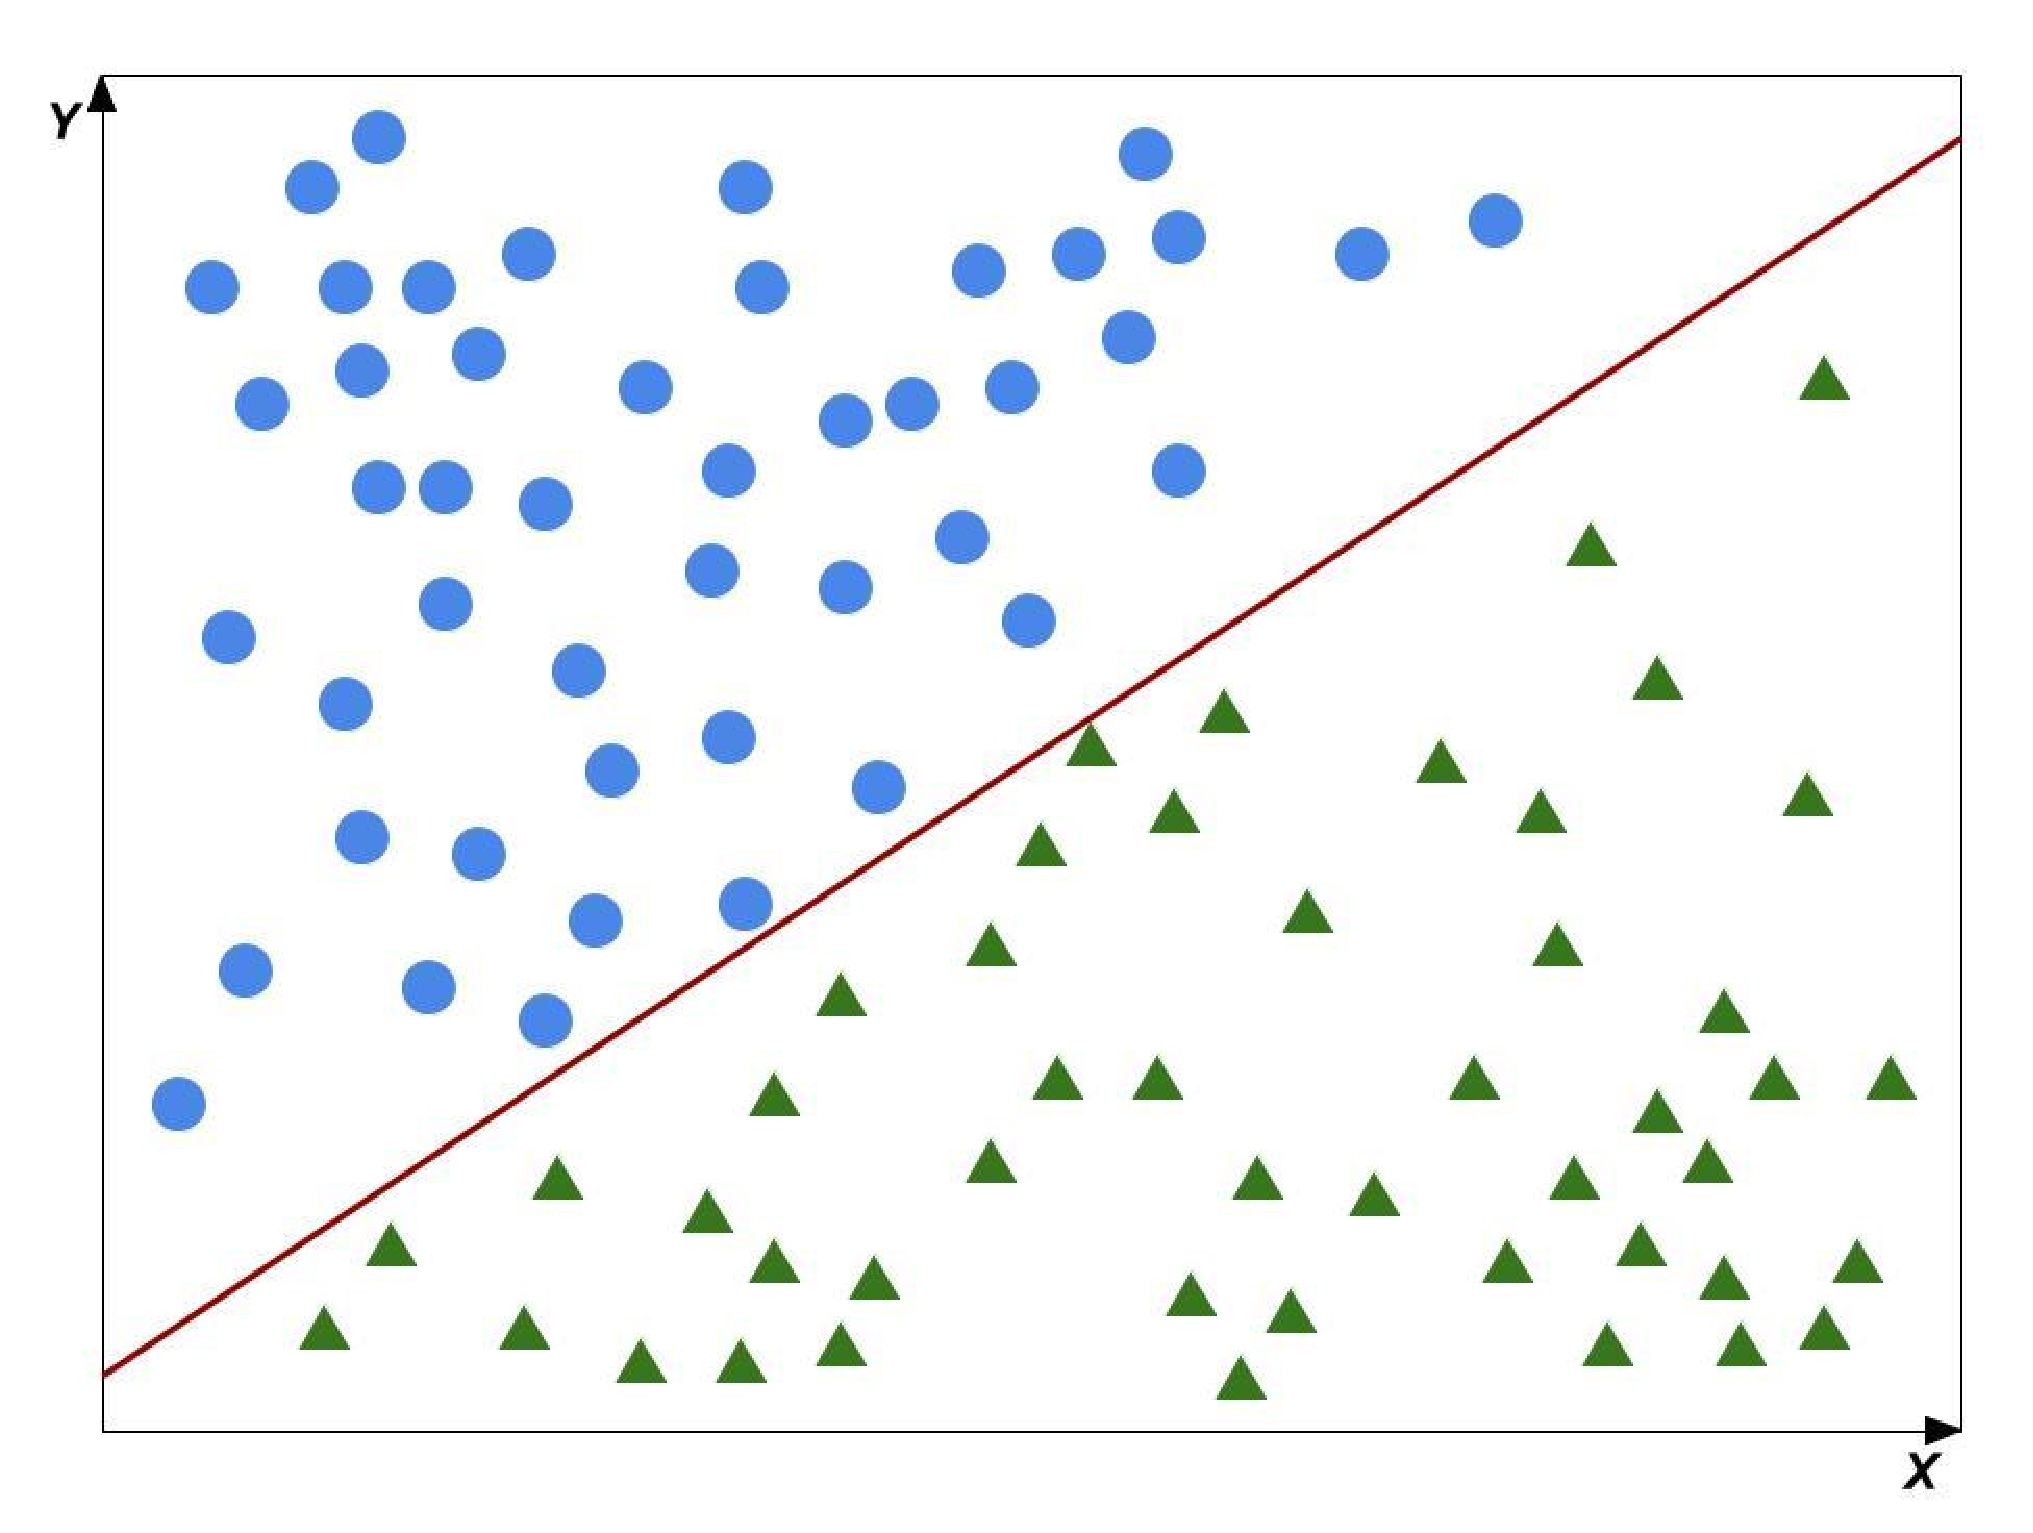
\includegraphics[width=\linewidth]{images/conceitosbasicos02.eps}
  \caption{Exemplo de separador linear}
  \label{fig:conceitosbasicos02}
\end{figure}

Com isso o problema se resume a calcular os valores do vetor de pesos \textit{w}.
Consideremos que temos disponível os dados dos diversos exemplos de círculos e triângulos vistos na figura.
A massa de exemplos envolvida no processo de aprendizado é denominada de \textit{conjunto de dados}.
Cada exemplo contém as coordenadas \textit{(x,y)} mais o valor da classe (circulo ou triângulo).
O algoritmo supervisionado simples proposto a seguir para resolver este problema é baseado no perceptron.
\\

\hline
\textbf{Algoritmo de aprendizado}
\hline
\hfill \break
Para cada exemplo do conjunto de dados:
\begin{enumerate}
\item Inicializa o vetor \textit{w} com valores aleatórios
\item Calcula o valor de saída de \textit{f(x)}
\item Verifica a diferença entre o valor obtido e o real (retirado do exemplo) e corrige os valores do vetor de pesos \textit{w} por fatores baseados nesta diferença
\end{enumerate}
\hline
\hfill \break

O perceptron é um algoritmo de aprendizado supervisionado clássico encontrado na literatura.
Ele serviu como base para outros algoritmos mais complexos como por exemplo o \textit{Support Vector Machine} (SVM).
Entretanto, existem algoritmos baseados em outros princípios.
Quando realizamos os experimentos deste trabalho procuramos comparar classificadores com princípios de funcionamento distintos.
Foram usados os classificadores: SVM, \textit{Nayve Bayes}, Arvore de Decisão, \textit{Random Forest} e \textit{k-nearest neighbors} (KNN).

No exemplo todos os atributos eram números reais.
Porém, com a utilização de outros algoritmos os atributos podem ser de diversos tipos: nominal (uma lista de classes), numérico (um número inteiro ou real), uma data, etc.

As tarefas de aprendizado supervisionado mais clássicas são a classificação, vista no exemplo, e a regressão.
Quando o alvo da tarefa é um atributo nominal dizemos que esta é uma classificação e quando é um número real dizemos que é uma regressão.
Todavia existem outras tarefas nas quais o aprendizado supervisionado pode ser empregado, como é o caso do \textit{ranking}.

Em um problema de \textit{ranking}, queremos que o modelo gere uma lista ordenada de classes como saída.
Para tanto, os exemplos fornecidos ao algoritmo de aprendizado também devem ter uma lista ordenada de classes ao invés de um atributo classe único.
Isto é, em cada exemplo $ (x_i,\; y_i) $ temos que $y_i$ é da forma $ [l_1, l_2, ..., l_k] $ onde \textit{k} representa o número total de classes. Veremos em outros capítulos que esta dissertação de mestrado se concentra em problemas desse tipo.

\subsection{Avaliação de performance}

Para treinar e avaliar a performance de um algoritmo de aprendizado, tipicamente o conjunto de dados é dividido em dois.
O primeiro, \textit{conjunto de treino}, contém os exemplos que efetivamente serão usados para treinar o algoritmo.
O restante, \textit{conjunto de testes}, é usado para fornecer exemplos inéditos ao modelo.
O resultado obtido quando o conjunto de testes é submetido ao modelo é utilizando para calcular as métricas pertinentes.
Essa divisão de dados é feita para garantir que o modelo foi capaz de generalizar e não apenas decorou o conjunto de dados (\textit{overfitting}).
Note que esta técnica de avaliação acaba por não utilizar uma parte dos dados (conjunto de teste) no treinamento.
Isso pode criar dificuldades quando a quantidade de dados disponível for muito limitada.

Outra forma de avaliação importante é chamada \textit{validação cruzada}.
Neste caso o conjunto de dados é dividido em \textit{k} subconjuntos.
Estes podem ou não manter aproximadamente as mesmas proporções de classes do conjunto de dados original, dependendo do que se deseja fazer.
A partir disso o algoritmo de aprendizado é executado \textit{k} vezes, gerando um modelo diferente por vez.
A cada iteração, aquele modelo é treinado com \textit{k-1} subconjuntos como conjunto de treino e o restante (1 subconjunto) como conjunto de testes.
Desta forma, no decorrer das \textit{k} iterações do treinamento, todos os dados são usados.
Por fim, os resultados de todos os modelos são combinados para gerar as estatísticas finais.

\section{O Framework Weka}

Neste trabalho utilizamos o Framework \textit{Weka} para construir o metaclassificador que implementa nosso método proposto. 
O \textit{Weka} é uma coleção de algoritmos de aprendizado para tarefas gerais de mineração de dados \cite{Hall}.
Ele contém ferramentas de pre-processamento, classificação, regressão, clusterização, etc.
Ele pode ser utilizado para aplicar os algoritmos aos dados por meio de sua interface gráfica ou pode ser chamado diretamente de um código Java.
